% !TEX root = ../Dokumentation.tex
\section{Realisierung}

\subsection{Raspberry Pi}

Folgende Installation \& Grundkonfigurationen müssen zu Beginn am Raspberry Pi vorgenommen werden.

\subsubsection{Software}
Die 32GB grosse SD-Karte welche man für das Raspberry benötigt, wird zu Beginn formatiert, um danach eine saubere Installation des Betriebssystems durchzuführen. Als OS wird die Version 2017-04-10 raspbian-jessie verwendet, dieses Betriebssystem wird von diversen Webseiten und Anleitungen empfohlen. Es hat eine graphische Oberfläche und bietet bereits vorinstallierte Programme.

\subsubsection{Konfiguration}
Nach der Installation der Software kann das Raspberry mit Maus und Tastatur an einen Monitor angeschlossen werden. Sobald das Raspberry mit Strom versorgt wird, startet der Boot-Vorgang.
Nun müssen alle wichtigen Grundkonfigurationen vorgenommen werden, auf dem vorliegenden Gerät folgendermassen umgesetzt:
\begin{itemize}
\item Tastatur: Deutsch(Schweiz)
\item Username: pi
\item Passwort: temperatur2017
\item Inteface SPI: enable
\item Netzwerk: aktuell ist die IP-Adresse fix mit 10.25.0.7 konfiguriert. Die IP sollte auf dem Raspberry Pi immer gleich bleibend sein, um das Gerät mit ssh erreichen zu können. Dies kann auch über eine Reservierung im DHCP Umfeld erreicht werden.
\end{itemize}

Die Sicherheitsrichtlinien auf dem Raspberry Pi sind tief, so ist der Standarduser pi Administrator und kann root Befehle ohne eingabe eines Passwortes ausführen. Dies sollte in einer sensitiven Umgebung entsprechend angepasst werden, dies ist allerdings ausserhalb des Scopes dieser Arbeit.

\subsubsection{Webserver}
Auf dem Raspberry wird zusätzlich ein Webserver bereitgestellt, damit die Temperaturausgabe direkt im lokalen Netz betrachtet werden kann. Als Webserver wurde Apache2 installiert.

\subsection{Softwaredesign}

Das Klassendiagramm (Abbildung \ref{fig:classdia}) bietet eine detaillierte Übersicht der Softwarelösung. Im Zentrum steht dabei die Klasse \code{Controller}, welche für die Sensoren, das XML-Handling sowie der Ausgabe benötigter Meldungen zuständig ist. Die digitalen Sensor- Rohdaten werden von der Klasse \code{SPIDataHandler} ermittelt, und vom \code{RawDigitalValueServer} bereitgestellt.

\begin{figure}[H]%Position festigen
\centering
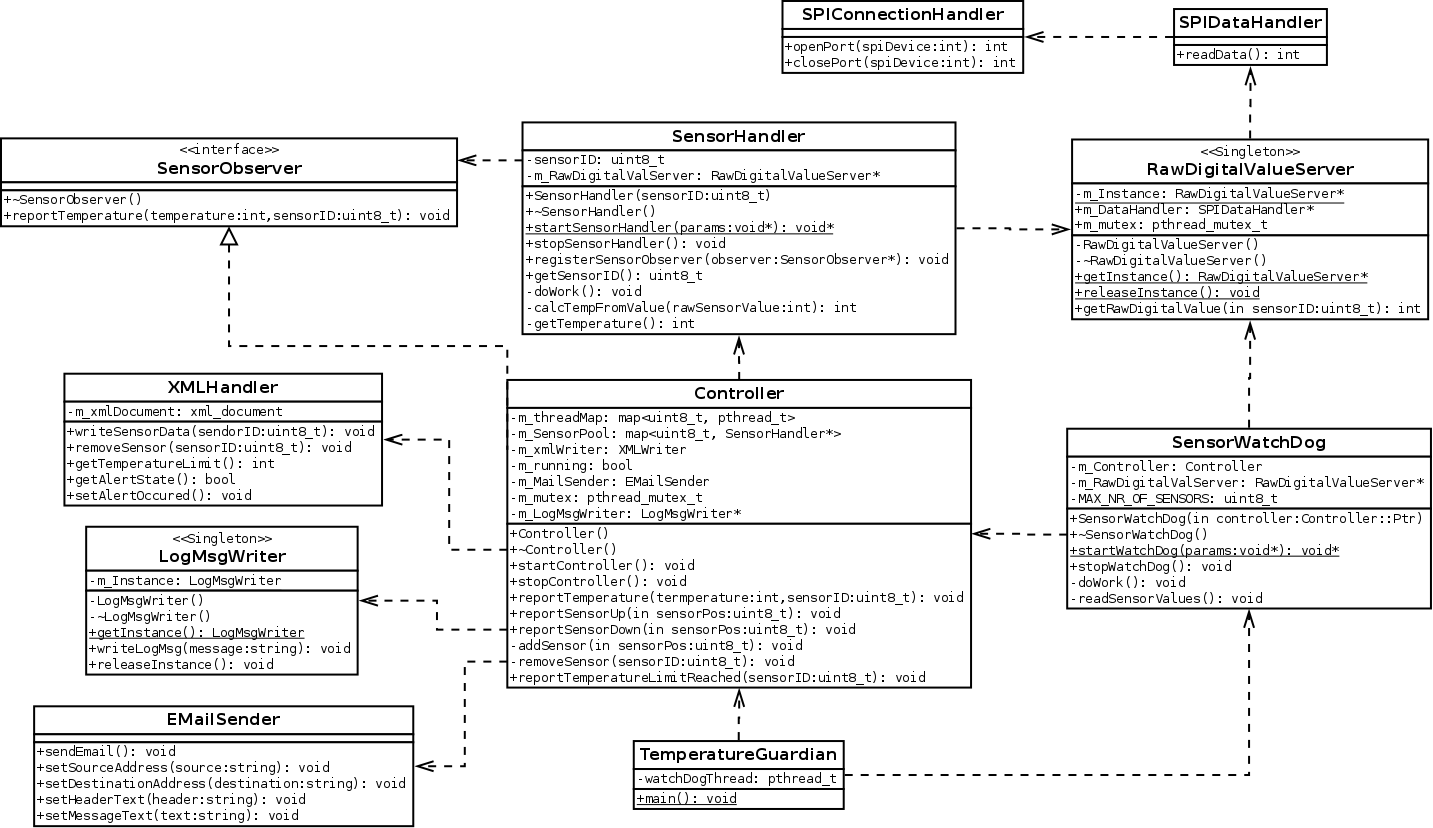
\includegraphics[width=1\textwidth]{Images/Klassendiagramm.png}
\caption{Klassendiagramm Software}
\label{fig:classdia}
\end{figure}

Die Klasse \code{SensorWatchDog} ist dafür zuständig, die angeschlossenen Sensoren zu prüfen, wird ein neuer Sensor angeschlossen, so wird dies dem Controller mittels der Methode \code{reportSensorUp} bekannt gegeben. Der Controller erzeugt dann einen neuen \code{SensorHandler} und startet einen Thread. Die Klasse \code{SensorHandler} überprüft und berechnet nun laufend die Temperaturwerte und rapportiert diese über den \code{SensorObserver} dem \code{Controller}. Der Wert des Sensors wird schlussendlich mittels \code{XMLHandler} in das File sensordata.xml geschrieben. Dieses File wird für die Ausgabe auf der Webseite verwendet.
Ebenfalls gibt es eine Logger-Klasse, welche alle Meldungen mit einem Zeitstempel ausgibt. Die Ausgabe erfolgt auf der Konsole und kann beim Aufruf des Programmes entsprechend in ein Logfile umgelenkt werden. So kann genau überprüft werden, wann ein Sensor angeschlossen oder entfernt sowie ob zum richtigen Zeitpunkt ein Mail versendet worden ist.

\subsubsection{Konfiguration und Sensorwerte}
Die XML Datei \code{sensordata.xml} ist sowohl Konfigurations- wie auch Ausgabedatei für die Sensorwerte.

\lstinputlisting[language=Xml]{04_Versuch/sensordata.xml}

Unter \code{SensorValues} ist ersichtlich, dass aktuell drei Sensoren angeschlossen sind und funktionieren, wobei bei einem abbruch des Programms die Werte nicht zurückgesetzt werden. Unter \code{LockedSensors} können alle Sensoren eingetragen werden, die nicht aktiv sein dürfen, da sie sich auf jenen Positionen befinden, die nur über das, in Kapitel 4.3 beschriebene, Spezialkabel angeschlossen werden können. Das Sperren der Sensoren ist notwendig, da sonst Störsignale auftreten. Unter \code{EMailSettings} lassen sich Ziel- sowie Absenderadressen einstellen. Des letzte Bereich \code{Setting} ist zum Setzen des Temperaturlimits reserviert. Zudem befindet sich dort auch der Alarmstatus, welcher von der Software auf 1 gestellt wird, sobald eine E-Mail-Nachricht versendet wurde. Dieser Wert kann somit auch durch  ein Monitoringsystem überwacht werden, sollte beispielsweise der E-Mail-Verkehr ausfallen. Solange der Alarmzustand auf 1 steht werden keine weiteren Nachrichten versendet. Durch Zurücksetzen dieses Wertes auf 0 wird das System wieder in den Normalzustand versetzt. 

\subsection{Verwendete Hardware}

Die in Abbildung \ref{fig:plate} dargestellte Baseboard, des Herstellers Linkerkit, bietet eine universelle Plattform, um verschiedene Aktoren anschliessen zu können. Für die verwendeten, analogen Temperatursensoren stehen vier Anschlüsse zur Verfügung, wobei jeder Anschluss zwei analoge Kanäle abdeckt.

\begin{figure}[H]%Position festigen
\centering
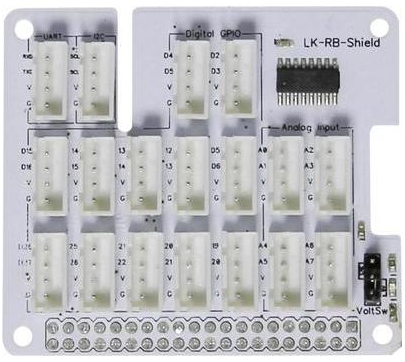
\includegraphics[width=0.25\textwidth]{Images/Basisplatine.jpg}
\caption{Basisplatine zum Raspberry Pi (Quelle www.Conrad.ch)}
\label{fig:plate}
\end{figure}

\begin{figure}[H]%Position festigen
\centering
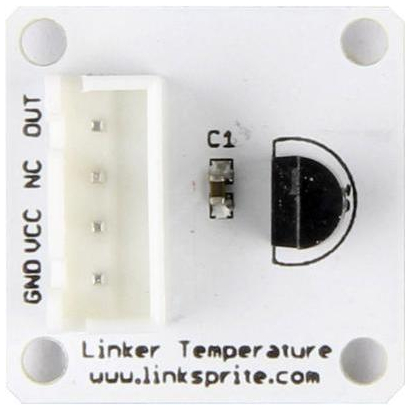
\includegraphics[width=0.25\textwidth]{Images/Sensorplatine.jpg}
\caption{Sensorplatine mit Temperaturfühler (Quelle www.Conrad.ch)}
\label{fig:sensor}
\end{figure}

Ein analoger Temperaturfühler auf einem passenden Board, in Abbildung \ref{fig:sensor} abgebildet, liefert Spannungswerte, abhängig von der Aussentemperatur. Diese Werte werden über den Analog- Digitalwandlerchip MCP3008, der sich auf dem Baseboard befindet in digitale Signale umgewandelt, welche mittels der Formel
\[
	T = 100 \cdot \left( \frac{D \cdot V}{1024} - 0.5 \right) 
\]
in Grad Celsius umgerechnet werden. Dabei entspricht $D$ dem digitalen Eingangswert, $V$ der Speisespannung für den Sensor, in unserem Fall 3.3V, und $T$ der resultierenden Temperatur.

\begin{figure}[H]%Position festigen
\centering
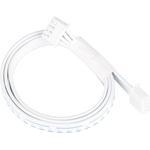
\includegraphics[width=0.25\textwidth]{Images/Verbindungskabel.jpg}
\caption{Verbindungskabel (Quelle www.Conrad.ch)}
\label{fig:cable}
\end{figure}

Die Sensoren werden mittels dem in Abbildung \ref{fig:cable} dargestellten Kabel verbunden. Um acht Sensoren anschliessen zu können, müssen spezielle Kabel angefertigt werden, da die Sensorplatine (Abbildung \ref{fig:sensor}) einen Anschluss nicht verwendet. Das dazu benötigte Schema ist in Abbildung \ref{fig:schema_doppelsensor} visualisiert. Wichtig ist dabei, auf allfällige Störfaktoren zu achten. Sämtliche Verbindungsstellen sollten zu den übrigen Verbindungsstellen abgeschirmt werden. Dieses Layout wurde im Rahmen dieser Arbeit nicht realisiert.

\begin{figure}[H]%Position festigen
\centering
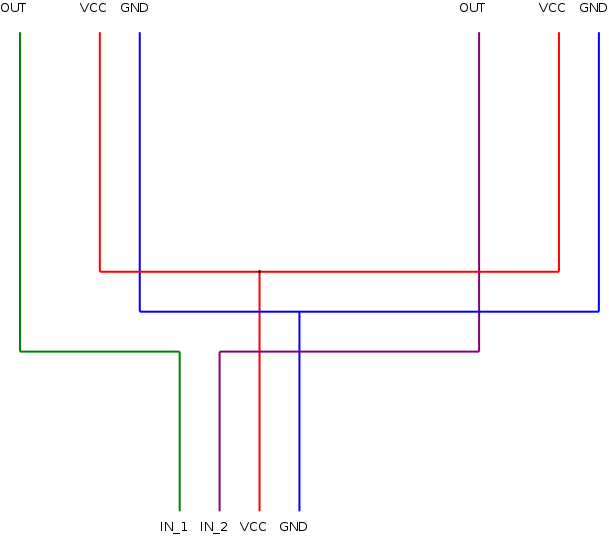
\includegraphics[width=0.25\textwidth]{Images/Schema.png}
\caption{Schema Verbindungskabel für zwei Sensoren}
\label{fig:schema_doppelsensor}
\end{figure}

\subsection{Webdarstellung}
Die Umsetzung der Webseite wurde hauptsächlich mit JavaScript gemacht.
Für die Anzeige der Temperatur wurde das JavaScript Plug-In JustGage verwendet. Diese visuelle Darstellung ermöglicht es, auf einen Blick zu erkennen, wie hoch die aktuelle Umgebungstemperatur ist. Zudem werden die Sensoranzeigen farblich hervorgehoben, sobald die Temperaturen in einen kritischen Zustand geraten.\\
Die Werte werden von der Software als XML-File geliefert, in welchem die Temperaturwerte sowie die ID pro Sensor gespeichert sind. Die Webseite wurde so konzipiert, dass dieses XML-File in einem regelmässigen Zyklus gelesen und die Temperaturwerte entsprechend auf der Seite ausgegeben werden. Dieser Punkt gehört mitunter zu einem der wichtigsten, denn die korrekte Anzeige der Temperaturwerte ist notwendig, um die Kontrolle jederzeit zu gewährleisten. Diese Anforderung kann mit \code {setInterval(function, 1000)} umgesetzt werden. Mit dieser Funktion werden die Temperaturwerte jede Sekunde oder nach Belieben neu vom XML-File gelesen.\\
Zusätzlich bringt JustGage eine Funktion mit sich, welche es ermöglicht über \code {refresh(val)} dem Sensor die neuen Werte zu übergeben. Wird ein Sensor angeschlossen, so sollte dieser zeitnah in das XML geschrieben und mittels \code {setInterval(function, 1000)} auf der Webseite ausgegeben werden. Auf der Webseite werden alle 8 Sensoren dargestellt. Wenn die Sensoren effektive an den GPIO's angeschlossen sind,  werden diese auf der Webseite als \grqq{}aktiv\glqq{} angezeigt. Im Gegenzug ist der Sensor \grqq{}inaktiv\glqq{} sobald dieser von der Basisplatine entfernt wird.\\
In der Funktion \code {readXMLNode(xml)} werden die Werte via \code{getEelemtsByTagName} aus dem XML gelesen und in ein Array gefüllt. Ist im XML der Sensor nicht vorhanden, so ist dieser entsprechend nicht angeschlossen und der Wert im Array wird mit 0 befüllt.\\

\textbf{Beispielcode der Webseite}\newline 
In dem folgenden Code wird eine Instanz des Sensors erstellt. In der Abbildung \ref{fig:sensor_webpage} ist die Darstellung mit einem aktiven Sensor und einer übergebenen Temperatur ersichtlich. 
\begin{lstlisting}{}
//Erstellen eines Sensors
var s1 = new JustGage({
	id: "s1",
	value: 0,
	min: 0,
	max: 75,
	title: "Sensor 1",
	hideMinMax: true
});
\end{lstlisting}

\begin{figure}[H]%Position festigen
\centering
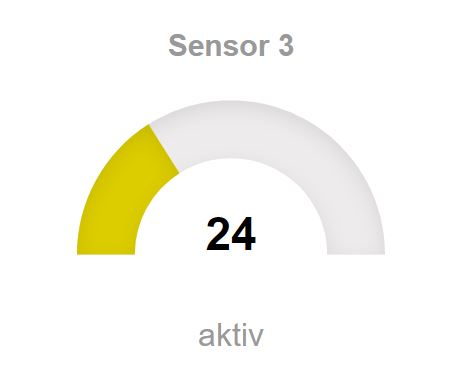
\includegraphics[width=0.25\textwidth]{Images/SensorWebseite.jpg}
\caption{Anzeige eines einzelnen Sensors}
\label{fig:sensor_webpage}
\end{figure}

Die untenstehende Funktion ist dafür zuständig, alle Sensorwerte aus der XML-Datei zu lesen. Zuerst wird mit einer for-Schleife durch das Array iteriert und jedem Index den Wert 0 zugewiesen. Anschliessend wird für jeden aktiven Sensor, Überprüfung mit \code{value > 0}, der aktuelle Wert dem Array übergeben.
\begin{lstlisting}{}
//Auslesen der Temperaturwerte
function readXMLNode(xml) {
	var xmlDoc = xml.responseXML;
	for (var i = 0, len = valueArray.length; i < len; i++) {
		valueArray[i] = 0;
	}                
	for (var i = 0, len = valueArray.length; i < len; i++) {
		sensorID = xmlDoc.getElementsByTagName("SensorValues")
		[0].getElementsByTagName("Sensor")[i].getAttribute("id");
		value = xmlDoc.getElementsByTagName("SensorValues")
		[0].getElementsByTagName("Sensor")[i].getAttribute("value");
		if (value> 0) {
			valueArray[sensorID] = value;
		}
	}
};
\end{lstlisting}

Im folgenden Codebeispiel wird das XML jede Sekunde neu geladen und über \code{s1.refresh(valueArray[0])} an den Sensor, welcher auf der Webseite angezeigt wird, übergeben. Im Array wird zusätzlich geprüft, ob der Wert null oder 0 ist. Ist dies der Fall so wird auf der Seite inaktiv ausgegben.

\begin{lstlisting}{}
//Zyklische Uebergabe der Temperaturwerte an den Sensor
setInterval(function () {
	loadXmlFile();
	s1.refresh(valueArray[0]);
	if (valueArray[0] != null && valueArray[0] > 0) {
		document.getElementsByClassName('container')[0].
		getElementsByClassName('t1')[0].innerHTML = 'aktiv';
	} else {
		document.getElementsByClassName('container')[0].
		getElementsByClassName('t1')[0].innerHTML = 'inaktiv';
	}
}, 1000);
\end{lstlisting}

\begin{figure}[H]%Position festigen
\centering
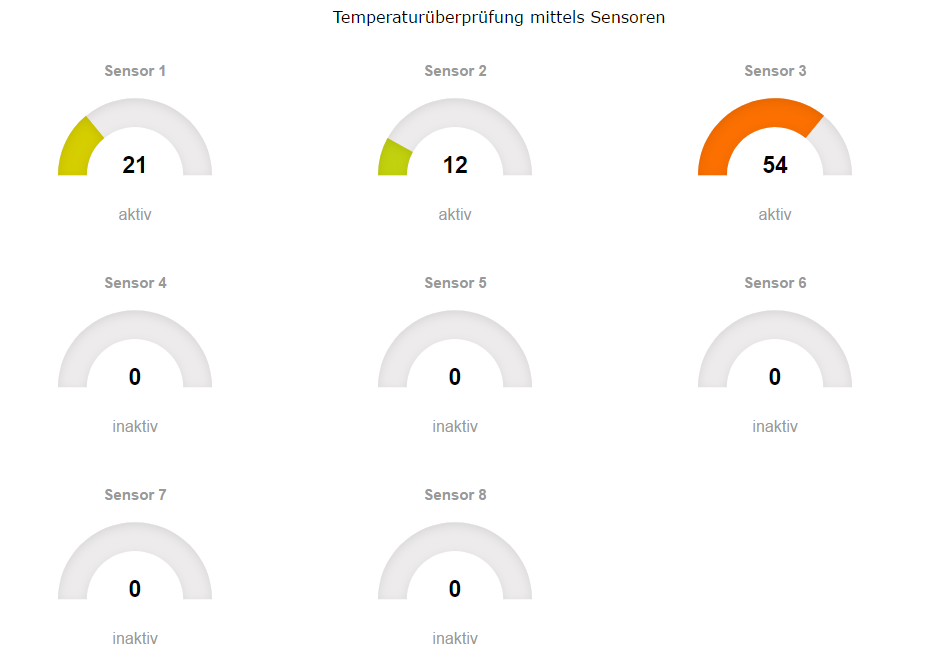
\includegraphics[width=0.75\textwidth]{Images/Webseite.png}
\caption{Ausgabe der Webseite}
\label{fig:webpage}
\end{figure}

\section{Versuchsdurchführung}
Testing war und ist während dem gesamten Realisierungsprozesses ein zentrales Thema. Zu Beginn wurde das Softwarekonzept lokal auf dem Notebook erstellt und schrittweise getestet, mittels Konsolenausgaben und simulierten Sensorwerten. So konnte das Konzept bereits vor Erhalt und Einrichtung des Raspberry Pi's geprüft und als funktionstauglich bewertet werden.\\
Die ursprüngliche Idee, die Umsetzung mittels automatisierter Tests abzusichern (Langr), musste aus Zeitgründen und fehlenden Erfahrungen fallengelassen werden.\\
Nach Abschluss der Einrichtarbeiten auf dem Raspberry Pi, wurden die Tests auf dem Gerät weitergeführt. Erst in kurzen Intervallen mit Beiziehen von vorhandenen Thermometern zu Hause und später in Langzeittests hat man die Software auf ihre Genauigkeit sowie ihre Resilienz gegenüber Abstürzen geprüft. Weiter ist auch das Hinzufügen und Entfernen von Sensoren wiederholt getestet worden. Das Versenden von E-Mailnachrichten ist mittels bewusstem Heruntersetzen der Grenztemperatur erfolgt. In diesem Bereich bestehen noch Berechtigungsprobleme, welche noch behoben werden.